\chapter{Force Estimation} \label{ch:fem}
In order to have a representation of the reaction force on the EndoWrist, estimation is needed. 
In \secref{introduction}, it is stated why force measurement can not be directly measured due to the lack of sensors. Thus the force has to be estimated by mathematical models as functions of actuator measurements.

The main challenge faced in making a model lies in the fact that the pulley system on the EndoWrist is nonlinear, and thus its full dynamics cannot be modeled in a straightforward manner. 
In other words, to have an accurate representation of Cartesian force a  nonlinear model is required.

One method of tackling this problem is to create multiple mathematical models pertaining to forces output by actions performed with the EndoWrist.
In this manner, the feedback vector is transformed from Cartesian space to a task space in which the chosen action forms a basis.\\
Each element of the new feedback vector corresponds to an actuated axis of the Geomagic Touch.

For the purpose of this project, we choose to feedback the yaw force generated by the grip action of the clamp, the torque generated by the roll actuator and force exerted by the clamps pitch movement.

\section{System Identification}
System identification is performed by fitting input and output data of the system to a known (grey-box) or unknown (black-box) mathematical model, generated either using theoretcal knowledge or data-fitting algorithms. 
This is done by changing the parameters of the model chosen, in such a way that the models error is minimized. 

For this project, it is required that the model outputs the force exerted by the EndoWrist.
%For our project, we require our model to output a measure of the force exerted by the EndoWrist.
Ideally a mathematical model derived from classical mechanics would be used to describe the dynamics involved in EndoWrist movement.
However, deriving this model precisely enough for grey-box identification has been proven difficult and time consuming due to the nonlinear nature of the dynamics\cite{kim2014dynamic}.

The nonlinearity of the EndoWrist dynamics emerges from friction forces between the pulley strings controlling the end-effector. This causes multiple pulleys to move in cases where only one actuator is actuated.
%This causes multiple pulleys to move in cases when only one is actuated. 
Additionally, the strings themselves are elastic, which adds another dimension of nonlinearity.

For these reasons it was decided to use a black box identification algorithms which only provide a general model structure where parameters do not have any physical meaning. 
Parameters are then identified using different variations of these algorithms and checked for accuracy.

The system identification process used in this project can be described in three steps:
\begin{enumerate}
\item Picking a model structure.
\item Identifying parameters.
\item Model validation.
\end{enumerate}

\subsection{Model structure}\label{se:ms}
The first choice regarding model structure pertains to linearity.
Since the system is nonlinear, a straightforward approach would involve choosing a nonlinear model structure for identification.
On the other hand, stability analysis of nonlinear models is difficult.\\
%Due to the nature of the system only a general trend in force is to be represented.
Since this project only aims for a trend representation of the force applied to the EndoWrist, it was decided to identify a linear state-space model which is used as a part of Hammerstein-Weiner nonlinear model \cite{zhu2002estimation}.

\subsubsection{State-space model}
A state-space model separates the dynamics of a system into a set of first-order differential equations.
Additionally, if the dynamical system is linear, time-invariant, and finite-dimensional, then the differential and algebraic equations may be written in matrix form. The general structure of such models is presented in \eqref{eq:ssc} and \eqref{eq:ssd} for the continuous and discrete variants, respectively.


\begin{equation}\label{eq:ssc}
\begin{split}
\dot{\mathbf{x}} &= \mathbf{A}\mathbf{x} + \mathbf{B}\mathbf{u} \\
\mathbf{y} &= \mathbf{C}\mathbf{x} + \mathbf{D}\mathbf{u}
\end{split}
\end{equation}

\begin{equation}\label{eq:ssd}
\begin{split}
\mathbf{x}(k+1) &= \mathbf{A}\mathbf{x}(k) + \mathbf{B}\mathbf{u}(k)\\
\mathbf{y}(k+1) &= \mathbf{C}\mathbf{x}(k) + \mathbf{D}\mathbf{u}(k)
\end{split}
\end{equation}



% \begin{align}\label{eq:ssc}
% \dot{\mathbf{x}} &= \mathbf{A}\mathbf{x} + \mathbf{B}\mathbf{u} \\
% \mathbf{y} &= \mathbf{C}\mathbf{x} + \mathbf{D}\mathbf{u}
% \end{align}
% \vspace{-0.5cm}
% \begin{align}\label{eq:ssd}
% \mathbf{x}(k+1) &= \mathbf{A}\mathbf{x}(k) + \mathbf{B}\mathbf{u}(k)\\
% \mathbf{y}(k+1) &= \mathbf{C}\mathbf{x}(k) + \mathbf{D}\mathbf{u}(k)
% \end{align}

This representation of a system is especially useful in linear MIMO systems as it maintains the same form for any number of inputs and outputs, as opposed to transfer functions.

\subsubsection{Hammerstein-Wiener model}
An identified state-space model can be used as the linear part of an Hammerstein-Weiner model, see \figref{weiner}.
Hammerstein-Wiener models are useful when the output of the system depends nonlinearly on its inputs, in this case it is possible to decompose the system into linear and nonlinear parts. 
The nonlinearity estimators at the inputs and outputs of the system can be modeled by a variety of nonlinear systems, e.g deadzones, saturations or neural networks.

\begin{figure}[H]
\resizebox{\textwidth}{!}{
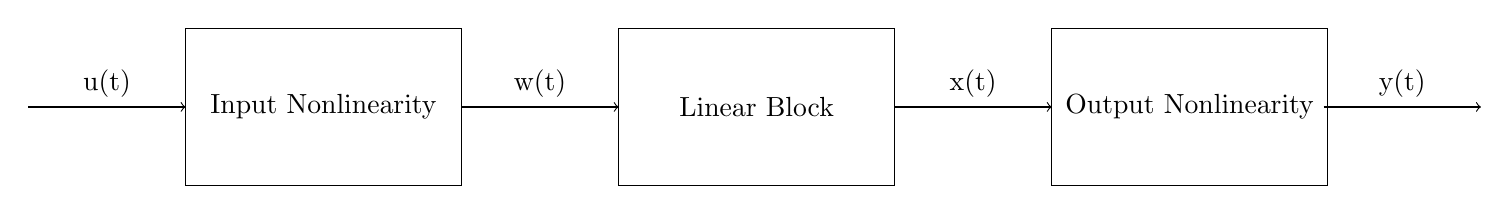
\begin{tikzpicture}
\draw  (-3.5,3) rectangle (0,1) node[pos=.5] {Linear Block};
\draw  (-9,3) rectangle (-5.5,1) node[pos=.5] {Input Nonlinearity};
\draw  (2,3) rectangle (5.5,1) node[pos=.5] {Output Nonlinearity};
\draw [->] (-5.5,2) -- (-3.5,2) node [pos=0.5,above] {w(t)};
\draw [->] (-11,2) -- (-9,2) node [pos=0.5,above] {u(t)};
\draw [->] (0,2) -- (2,2) node [pos=0.5,above] {x(t)};
\draw [->] (5.45,2) -- (7.45,2) node [pos=0.5,above] {y(t)};
\end{tikzpicture}
}
\caption{Block diagram of a Hammerstein-Wiener model.}
\label{weiner}
\end{figure}

A deadzone nonlinearity is used for this project to represent the friction effect on the force.
Different output nonlinearities are also utilized and compared.
% A deadzone nonlinearity on the input allows us to represent the effects of friction on the force, and is used in this model.
Different output nonlinearities are also utilized and compared.
\todo{Filip?}

\subsubsection{Inputs and outputs}
\todo{This section is more a discussion of next approch?}
Multiple approaches have been considered when taking into account inputs and outputs of the system.

The most direct approach would have all the available data as inputs to a single output system, which outputs a force estimate.
Ideally, this would provide enough information to identify an accurate force model.\\
However, the imperfect nature of measuring equipment and the experiments performed, as well as limits in computing power and optimization algorithms prevent a fully utilization of this information.

A more robust approach could be a system that estimates some measurable values in addition to force.\todo{don't understand this paragrapfh}
If the system is observable and the model captures the dynamics sufficiently, it could be possible to correct the model states using output errors.

Both of these approaches are examined and simulated in this chapter.

The same modeling process was used for both yaw and pitch force models, while the roll torque model is explained in section \ref{se:mdval}.
For clarity, the results of each step in the process will only be presented for the yaw model, while the final results will be presented for both the yaw and pitch models. 

\section{Parameter identification}\label{sec:para_iden}
%Once a general model structure has been chosen, parameter identification algorithms can be utilized.

For parameter identification to be performed on the Hammerstein-Weiner model, a linear model needs to be defined.
This means that it is first necessary to identify the linear state-space model of the system.
Linear state-space model fitting can be done using various methods, but for this purpose it has been chosen to use a subspace identification algorithm.
%we have chosen the subspace identification algorithm.

Subspace identification is an algorithm that combines concepts from system theory, linear algebra and statistics in order to provide a state-space model of the system, which makes it useful for MIMO system identification \cite{van2012subspace}. 
The most important achievement in subspace identification is that Kalman filter states can be obtained from input-output data using linear algebra methods.
Although the algorithm itself is complex, it is implemented in the System Identification Toolbox as a part of MATLAB.

One advantage of subspace identification algorithms is the ability to estimate how much of the data dynamics a state-space model of a certain order can represent. 
As seen on figure \figref{fig:ssid1}, the diminishing returns of increasing the state-space order are visible for different subspace identification algorithms.\todo{This line?}

%figure of subspace singular value analysis

\subsection{Identification data}
\todo{In gerneal we need a concluding text to each figure}

Both approaches discussed in \secref{se:ms} are possible to realize on the data sets acquired in \chapref{cha:measurement}.
However, the data contains various irregularities caused by the imperfect measuring process as well as the hardware. 
For this reason, parts of the data needed to be removed before identification, which required interpretation of results.

\todo{This paragraph}
Noise is also present and can be removed from the identification data using a low pass filter.
Since most of the dynamics are captured in the frequency band of 0 to 20 Hz, this frequency range was chosen for identification.
Offsets were also removed from the output data as they reduced model quality.
A sample of original and modified data can be seen on \figref{figlowpass}.

\begin{figure}[H]
\centering
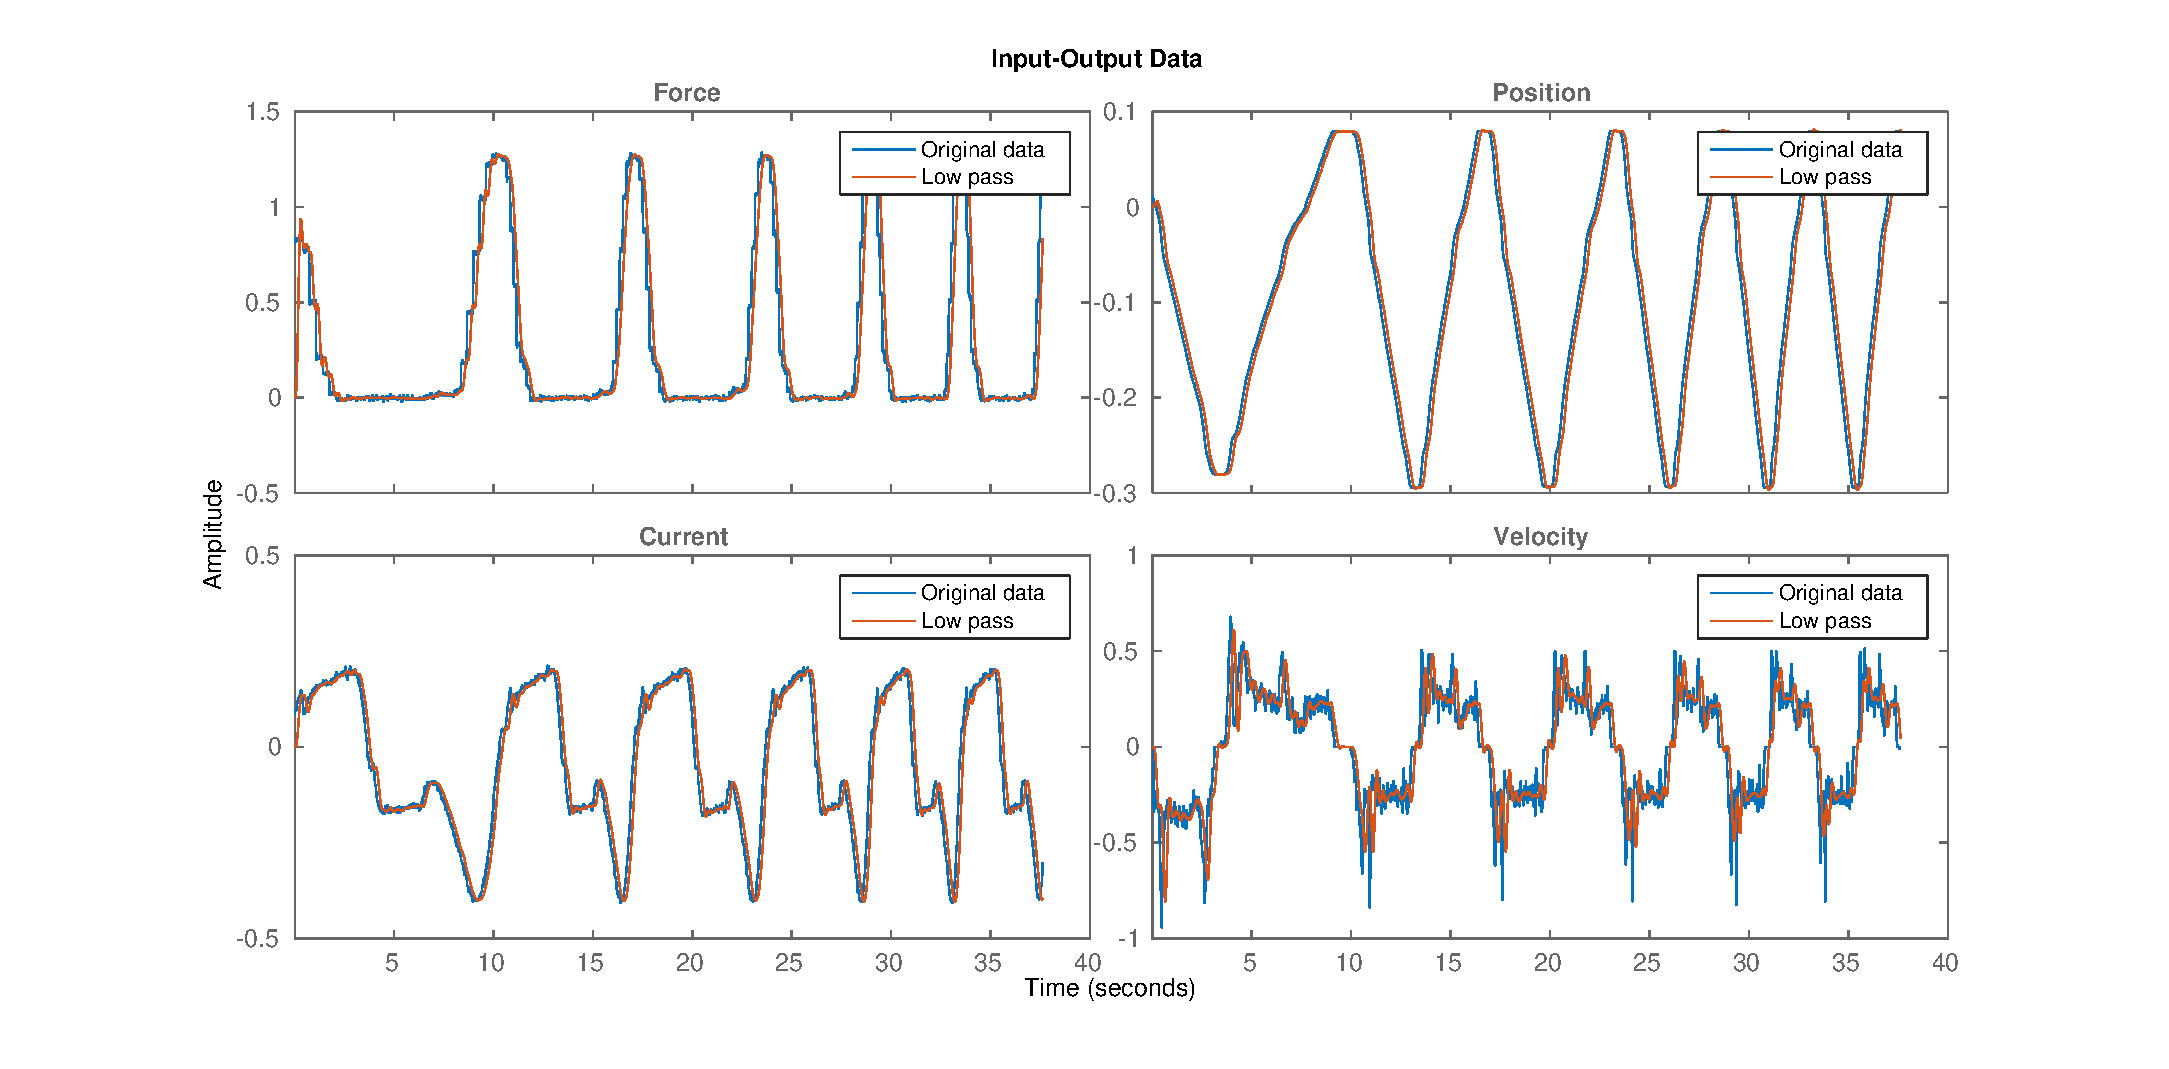
\includegraphics[width=\textwidth]{lowpass.eps}
\caption{Comparison of original and low-pass filtered data.}
\label{figlowpass}
\end{figure}

Linear models can also be fitted in the frequency domain so the data is transformed using fast Fourier transform \cite{van1992computational} and used in the identification process.

\subsection{Linear model identification}
The System Identification Toolbox provides three different subspace identification algorithms which often provide different results depending on the chosen system order \cite{van1994n4sid}. 
For this reason all 3 algorithms are attempted in the identification process, and the best one is chosen depending on the average fit.
The algorithm which provides the best result varies heavily on the data set and the chosen order of the model, see \figref{fig:ssid1}.
It can be see that second order models have slightly different dynamics depending on the algorithms, while in certain cases some models lose stability.

\begin{figure}[H]
\centering
\hspace{-2em}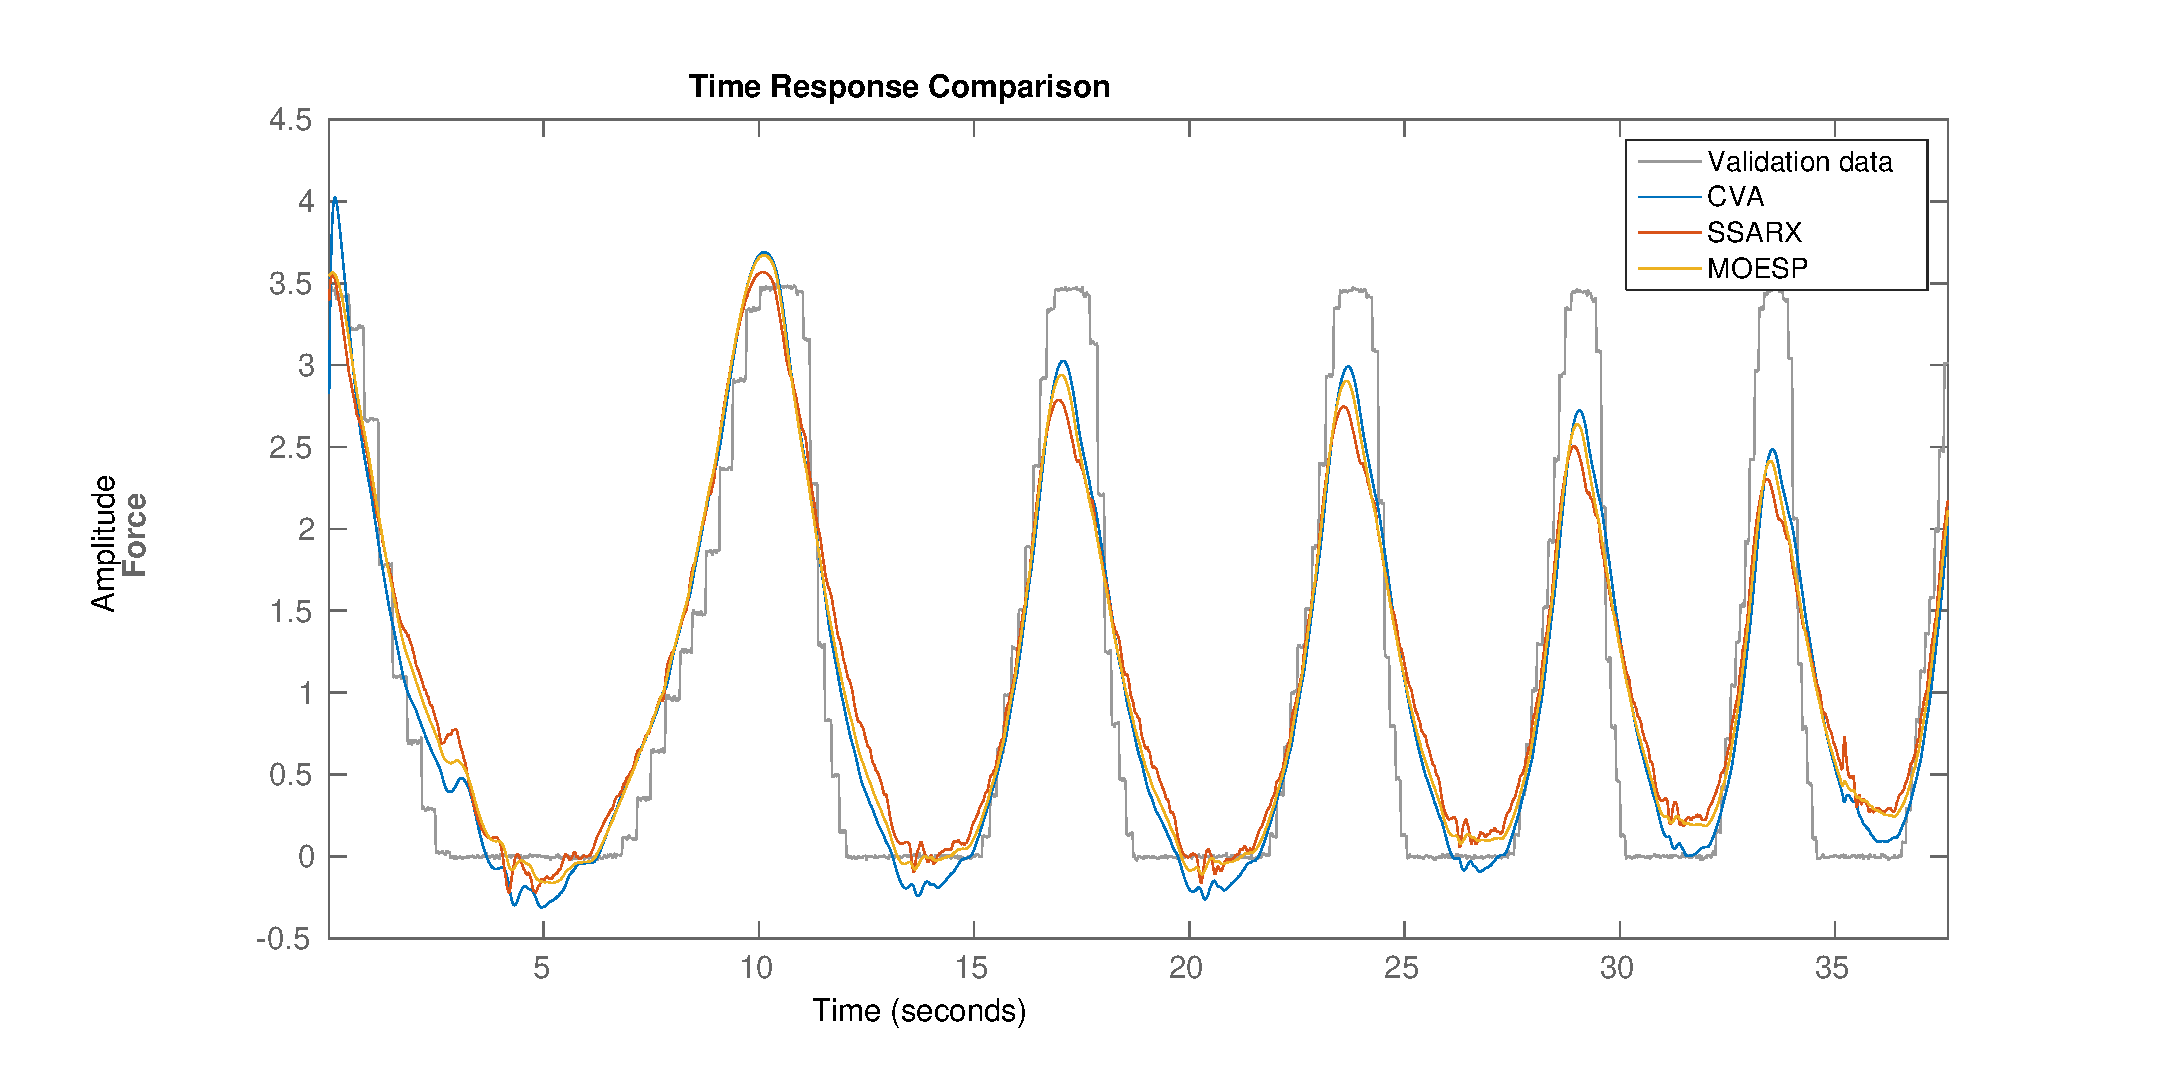
\includegraphics[width=\linewidth]{sscomparison1}
\caption{Second and sixth order yaw force models identified by different subspace identification algorithms. 
The lower plot shows only two methods as the SSARX method is not stable for this order and data set.}
\label{fig:ssid1}
\end{figure}

The choice of inputs, outputs and the domain of identification data heavily affects the model quality in a unpredictable way, see \figref{fig:fits}.
It is assumed that the cause of this is a limited number of iterations, since a higher order model should always represent dynamics better than a lower order one.

\begin{figure}[H]
\hspace{-2.5em}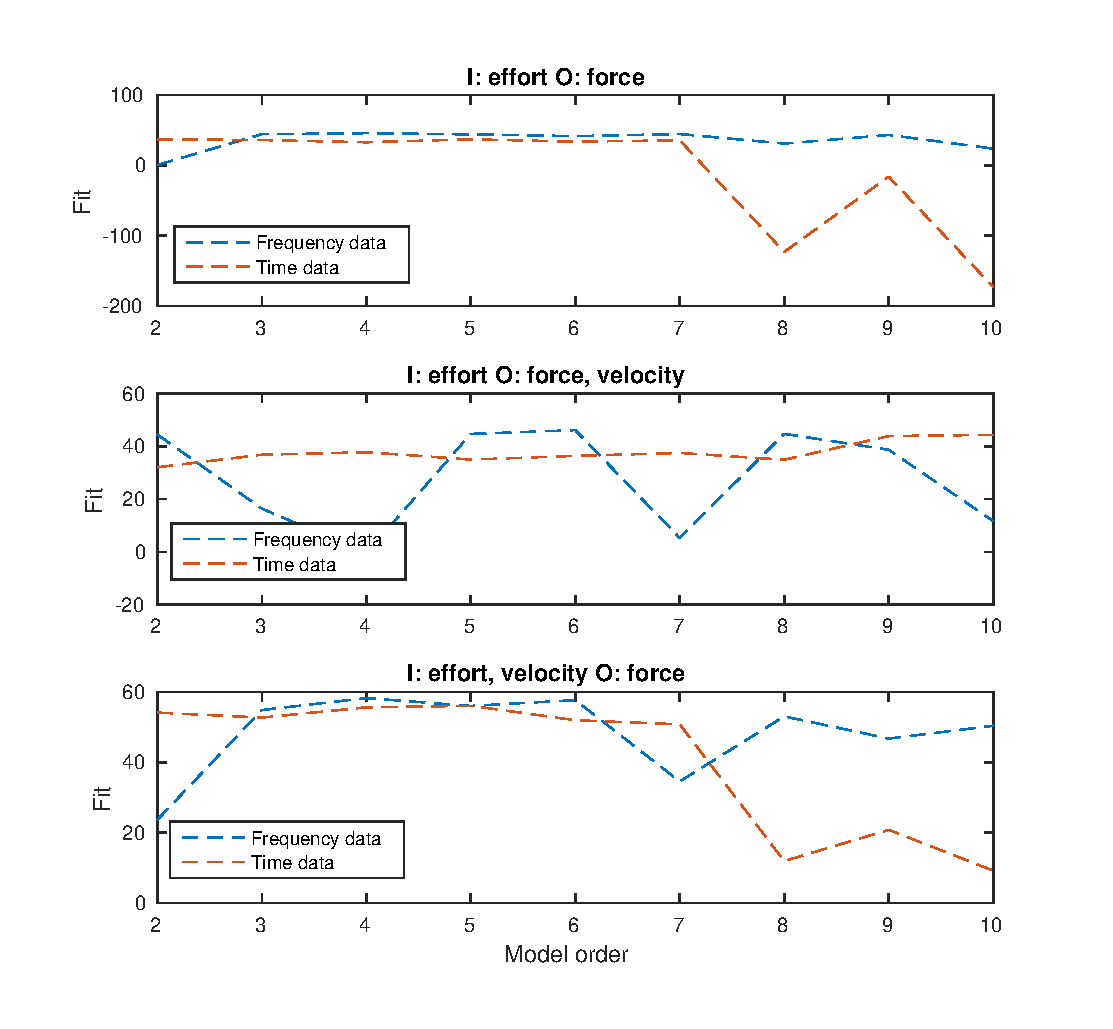
\includegraphics[width=\linewidth]{fits}
\caption{Best average fit of models to validation data depending on the order and domain of data used in identification.}
\label{fig:fits}
\end{figure}

This fact makes an approach consisting of testing various inputs and outputs  necessary in picking the best model for estimation.
Comparing the responses of these models it is clear that having effort and velocity as inputs provides a much better estimate than when the only input is effort.
As seen in \figref{fig:fits} his is true for both the time and frequency data sets.

\begin{figure}[H]
\centering
\hspace{-2em}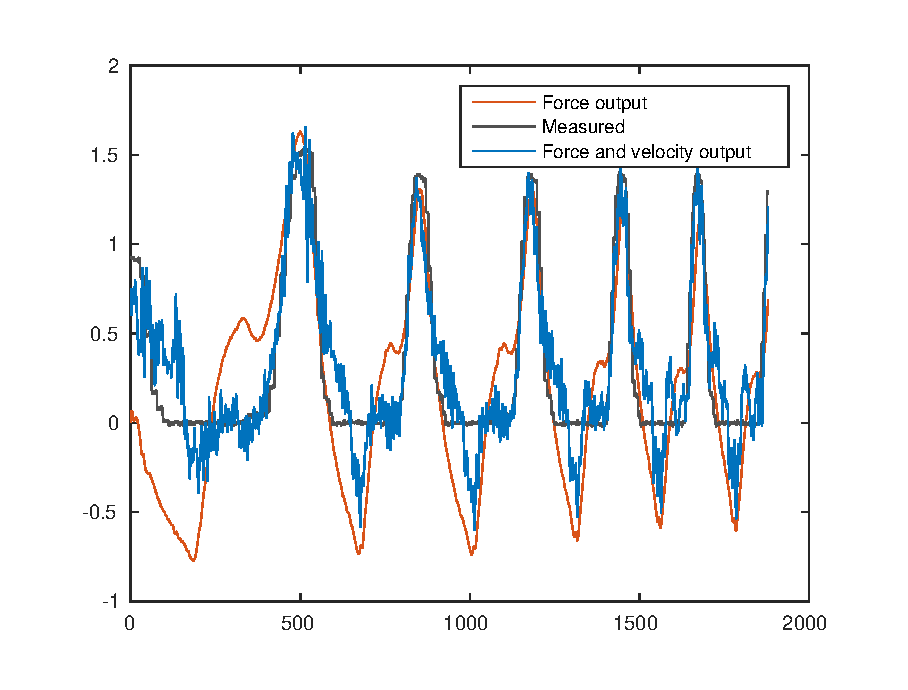
\includegraphics[width=\linewidth]{comparisonp1p2}
\caption{Second order yaw force models identified by different subspace identification algorithms.}
\label{fig:1LMI2}
\end{figure}



\subsection{Hammerstein-Weiner model identification}\label{hammerWeinmodeid}

A linear model is identified and the estimate of the deadzone nonlinearities with the Hammerstein-Wiener model can be made.

%Once the linear model is identified we can estimate the nonlinearities with the Hammerstein-Wiener model.

\begin{figure}[H]
\centering
\hspace{-2.5em}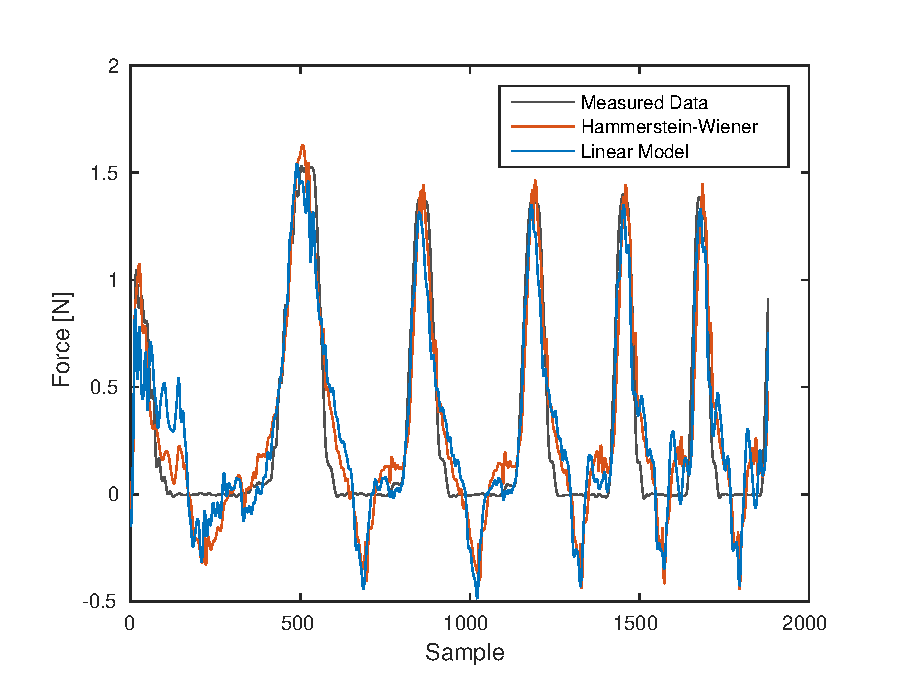
\includegraphics[width=0.7\linewidth]{sshwcomp1}
\caption{Hammerstein-Wiener model with deadzone nonlinearity responses compared to measured data for yaw force.}
\label{fig:2LMI}
\end{figure}

\begin{figure}[H]
\centering
\hspace{-2.5em}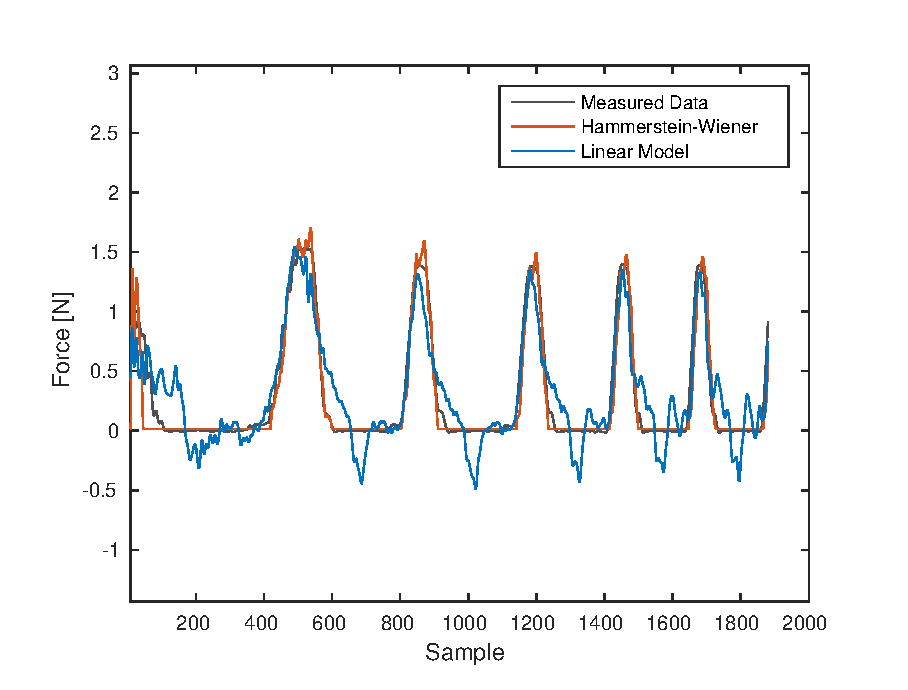
\includegraphics[width=0.7\linewidth]{sshwcomp2}
\caption{Hammerstein-Wiener model with deadzone input nonlinearity and saturation output nonlinearity responses compared to measured data for yaw force.}
\label{fig:2LMI1}
\end{figure}

\begin{figure}[H]
\centering
\hspace{-2.5em}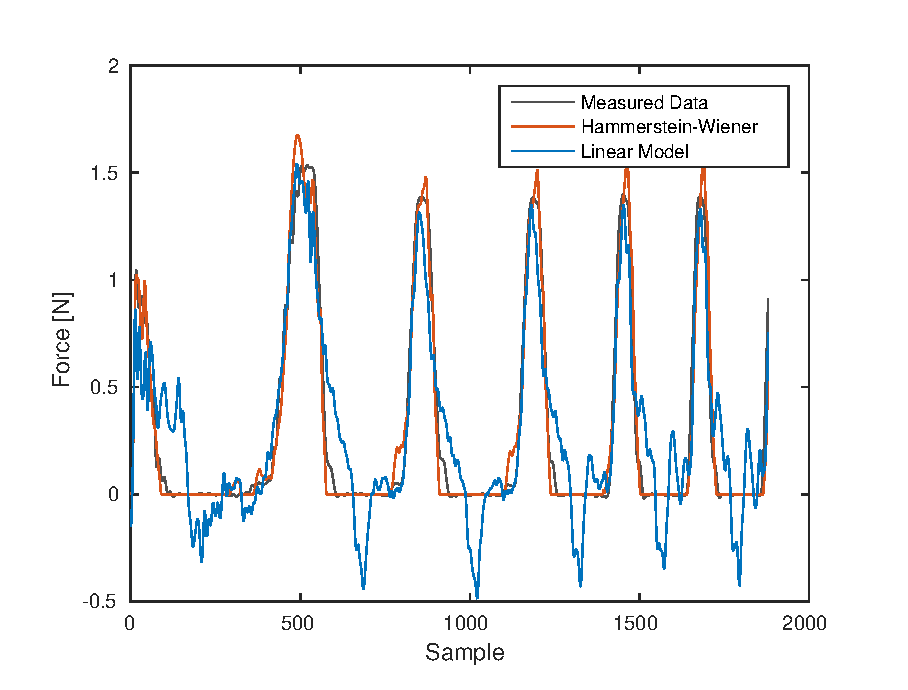
\includegraphics[width=0.7\linewidth]{sshwcomp3}
\caption{Hammerstein-Wiener model with deadzone nonlinearities on the output.}
\label{fig:2LMI2}
\end{figure}

From \figref{fig:2LMI}, \figref{fig:2LMI1} and \figref{fig:2LMI2} it should be noticed that the deadzone nonlinearity on the inputs significantly improves the linear model and as such makes for a good yaw force model.
This serves as a proof of concept for our own friction estimating nonlinearity based on measured data described in the control chapter.

\section{Model validation} \label{se:mdval}
In this section, the model derived in \secref{hammerWeinmodeid} is tested. This test is done on new data, which the model has not been fitted to.

%Once a model has been created, it needs to be tested on data it wasn't originally fitted to.

%We expect our model to capture the general force dynamics in a way that is proportional to the actual force.
%In that way we are able to represent the resulting force estimate as force feedback on the Geomagic Touch.

The model is expected to capture the general force dynamics in a way proportional to the actual force. If this is to be true, the represented force estimate can be send back to the Geomagic touch as force feedback.

It should be noted that the model is fitted to dynamics of a clamp gripping a load-cell, which has a hard surface, thus having a steep force gradient.
It is expected that soft tissue would have a much smaller force gradient, thus it is expected that the model response overestimates the force slightly.
%An important observation is that this model is fitted to dynamics of the clamp gripping the load cell, which has a hard surface.
%It is expected that soft tissue would have a much smaller force gradient and thus it is expected that the model response overestimates the force slightly.
\todo{don't know how to continue this}
Nonetheless, through the use of the system we came to a conclusion that the response is satisfactory for the degree of accuracy provided by the Geomagic Touch force feedback.

In \figref{fig:final_res_yaw} and \figref{fig:final_res_pitch} the response to different types of input data is examined.
The data was gathered in measurements described in chapter \ref{cha:measurement}, but wasn't used in the fitting process.


\begin{figure}[H]
\hspace{-3em}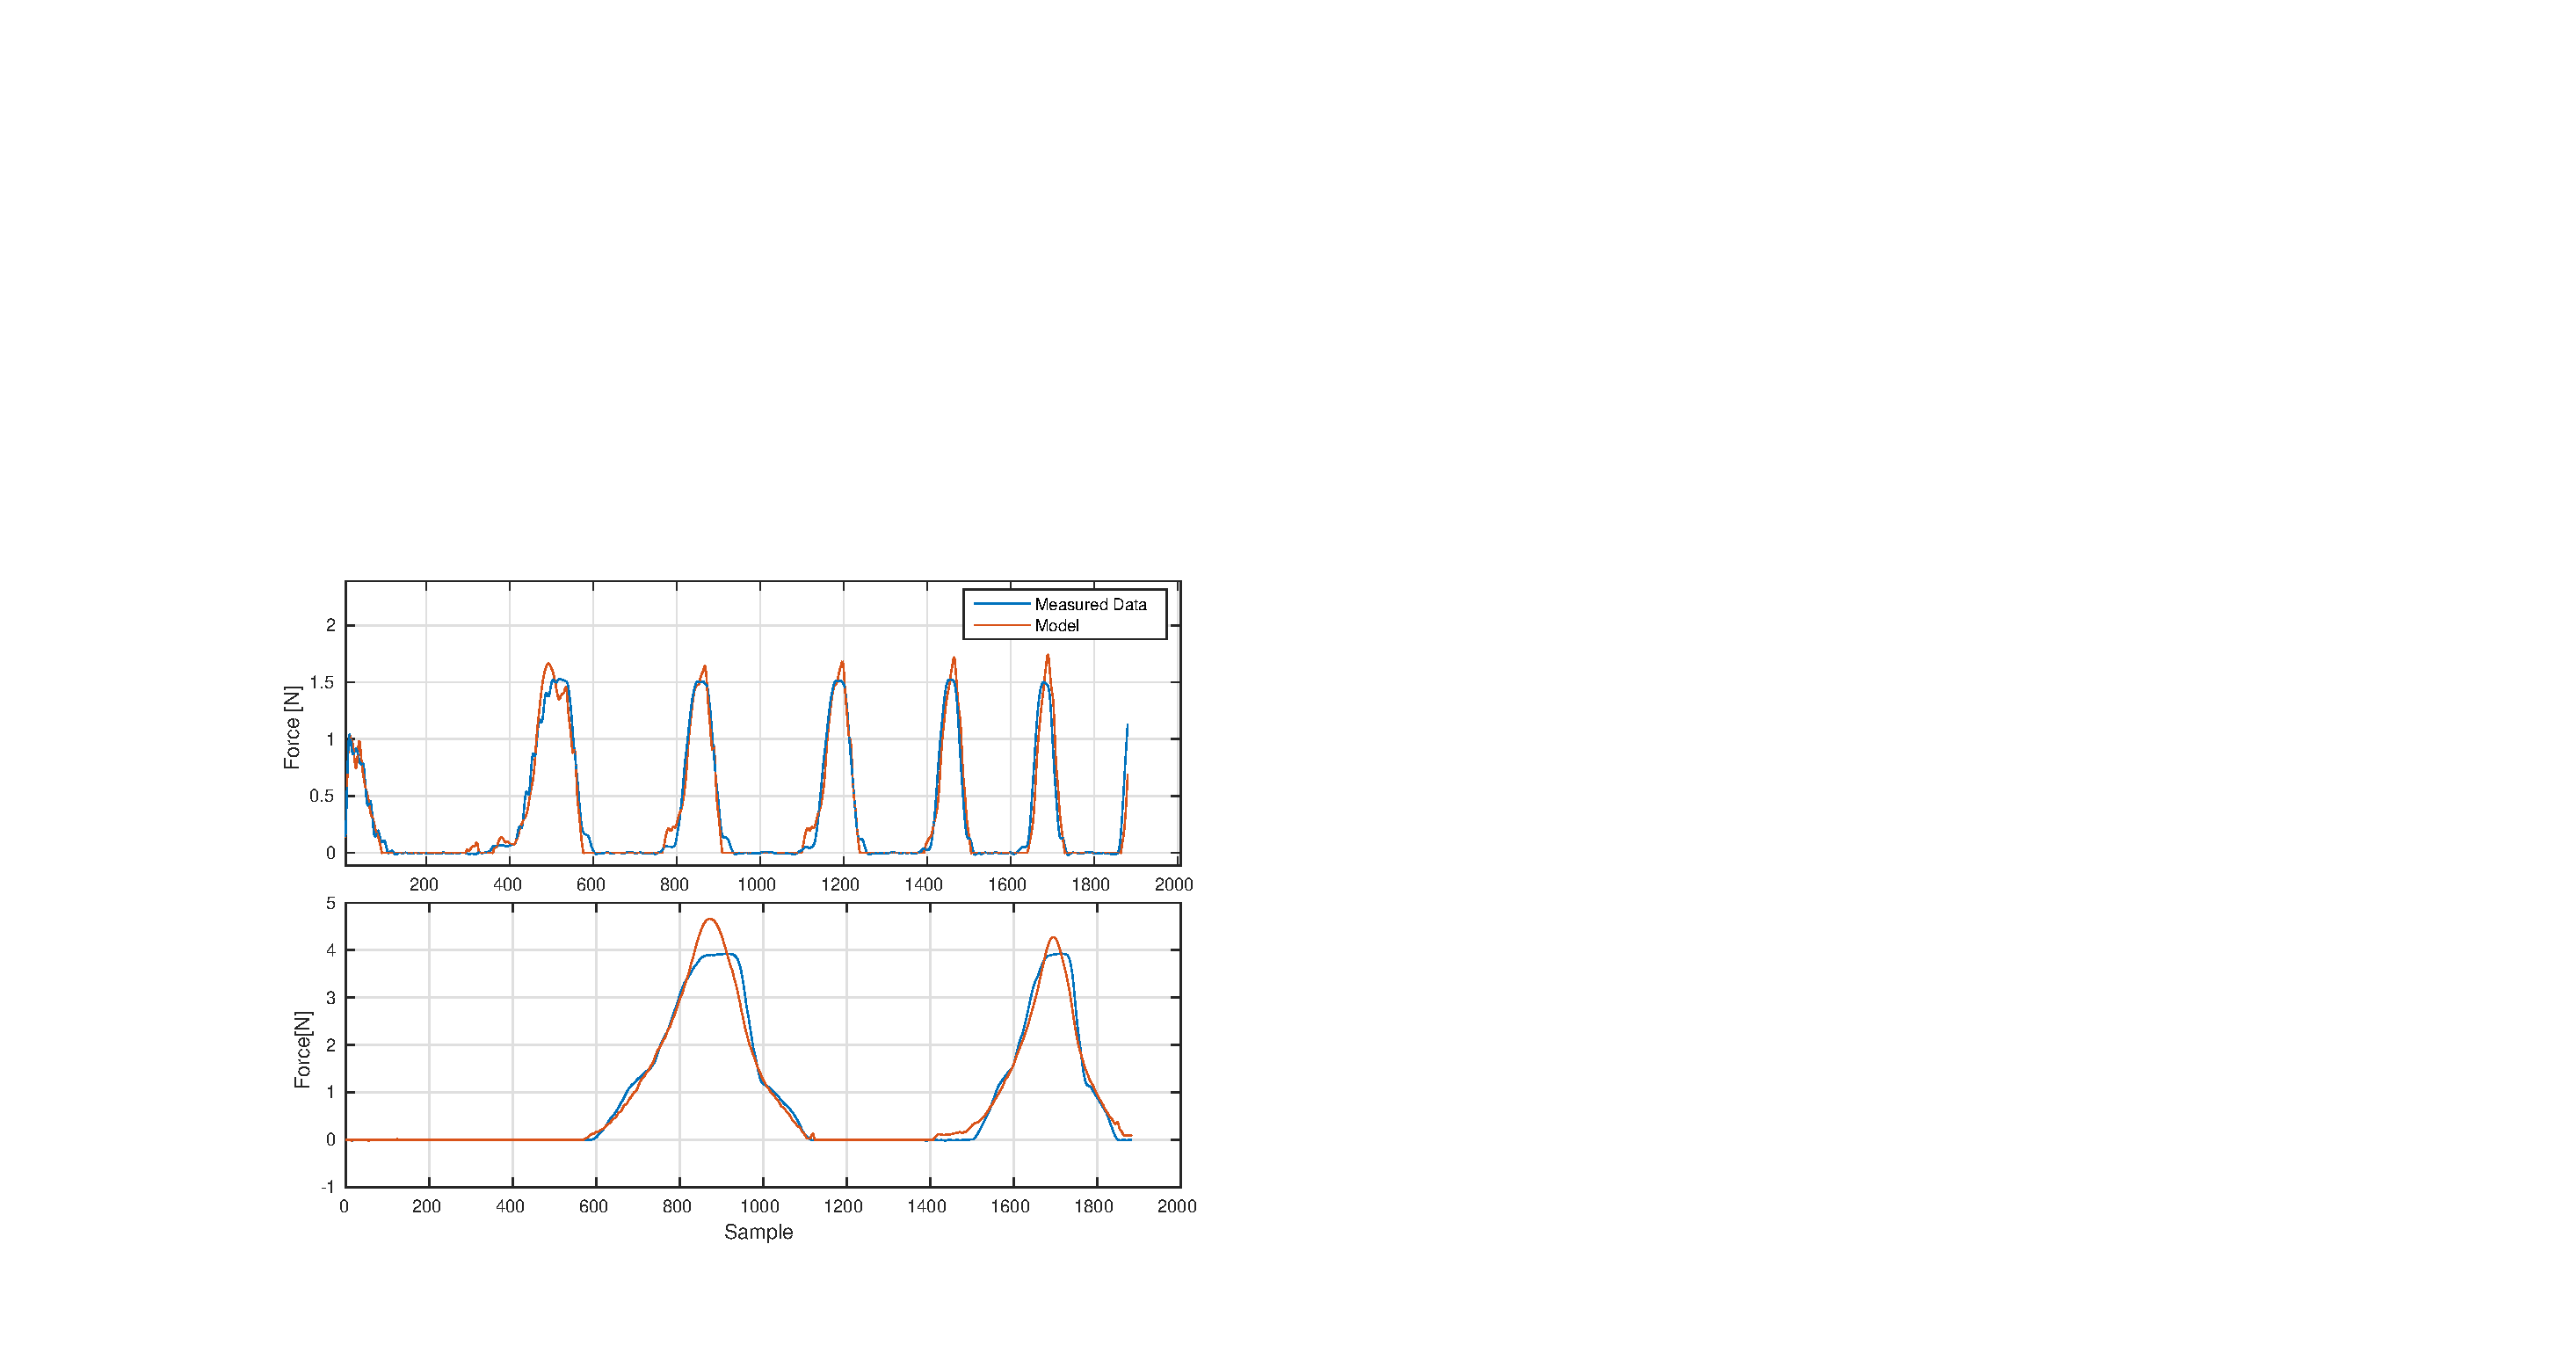
\includegraphics[width=1.2\linewidth]{modelyaw}
\caption{Yaw model excited with different types of inputs.}
\label{fig:final_res_yaw}
\end{figure}

Unlike the yaw model, the nonlinear pitch model had large jumps in value and was not useful for feedback.
Thus, the linear model is used in estimation until a better model is developed.

\begin{figure}[H]
\hspace{-2.5em}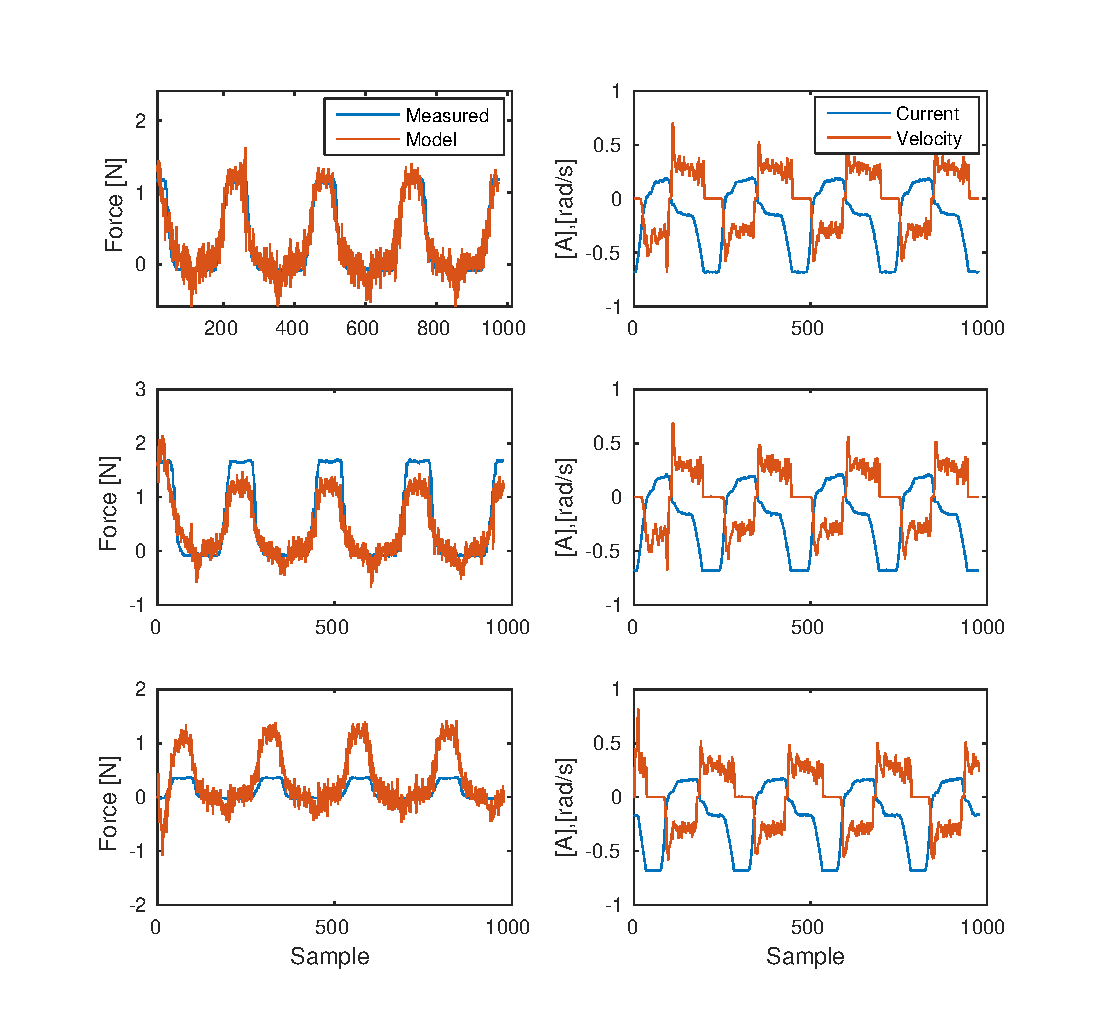
\includegraphics[width=1.2\linewidth]{modelpitch}
\caption{Pitch model excited with different types of inputs.}
\label{fig:final_res_pitch}
\end{figure}

The roll torque, which is determined by the roll actuator and directly rotates the entire tool, making it independent to the rest of the system.
We can model the roll torque as a state that only depends on input in the state space model of the system \ref{eq:allSS}.
The final model is derived by simple measurment, as described in \figref{fig:entire_force_testsetup} and \figref{fig:endeffector_force}.
%\begin{align}\label{eq: roll}
%F_{roll} = 20e_{roll}
%\end{align}

A  useful property of viewing the linear parts of models in the state-space is simple parallel composition.
This means that the entire dynamic model of the system can be viewed as one state space matrix (\ref{eq:allSS}).

\begin{align}\label{eq:allSS}
\mathbf{x}(k+1) &= 
\begin{bmatrix} \mathbf{0} & \mathbf{0} & \mathbf{0}\\
 \mathbf{0} & \mathbf{A}_{pitch} &\mathbf{0}\\
 \mathbf{0} &\mathbf{0} & \mathbf{A}_{yaw}  \end{bmatrix} 
 \mathbf{x}(k) + 
\begin{bmatrix} \mathbf{B}_{roll} & \mathbf{0} & \mathbf{0}\\
 \mathbf{0} & \mathbf{B}_{pitch} &\mathbf{0}\\
 \mathbf{0} &\mathbf{0} & \mathbf{B}_{yaw}  \end{bmatrix} 
 \mathbf{u}(k)\\
\mathbf{y}(k+1) &= 
\begin{bmatrix} \mathbf{C}_{roll} & \mathbf{0} & \mathbf{0}\\
 \mathbf{0} & \mathbf{C}_{pitch} &\mathbf{0}\\
 \mathbf{0} &\mathbf{0} & \mathbf{C}_{yaw}  \end{bmatrix} 
\mathbf{x}(k) 
\end{align}

This is a useful way to view the system since the force feedback loop can be veiwed as a single system with state feedback and input/output nonlinearities.

\section{State estimator design} \label{se:est}
As mentioned in section \secref{se:ms}, an approach was taken towards designing a state estimator which could correct the force estimates.
This method would involve designing a steady-state Kalman filter \cite{brown1997introduction} and/or a Luenberger observer \cite{friedland2012control} for a model that outputs both force and velocity.

The difference between the Kalman filter and the Luenberger observer is based on the fact that the Kalman filter takes into account the stochastic nature of measurements and processes. The Luenberger observer is based on deterministic systems and does not "weigh" data according to reliability.

Before implementing an observer/estimator, it is necessary to check the  systems observability.
Formally, a system is said to be observable if, for any possible sequence of state and control vectors, the current state can be determined in finite time.
The observability is found by ascertaining that the rank of the observability matrix \eqref{eq:obs} is equal to the rank of $\mathbf{A}$.
%We determine observability by ascertaining that the rank of the observability matrix (\ref{eq:obs}) is equal to the rank of $\mathbf{A}$. 

\begin{align}\label{eq:obs}
\mathcal{O}_v=\begin{bmatrix} C \\ CA \\ CA^2 \\ \vdots \\ CA^{v-1} \end{bmatrix}
\end{align}

Checking the matrices of the linear parts of our models, we find that this is indeed true and an observer gain exists.

\subsection{Kalman filter}
The Kalman filter is an estimation algorithm that uses a series of measurements observed over time to produce estimates of unknown variables in a system.
Estimation is carried out in two steps:

\begin{itemize}
\item Prediction step.
\item Update step.
\end{itemize} 

The prediction step consists of calculating \textit{a priori} estimates of the current state and covariance using the updated state estimates from the last step. \todo{don't understand}
The $\mathbf{P}$ matrix is the so called covariance matrix and represents the estimated accuracy of the state estimate.
The $\mathbf{Q}$ and $\mathbf{R}$ matrices represent the covariances of the measurement noise, respectively.

\begin{gather}
\hat{\mathbf{x}}_{k\mid k-1} = \mathbf{A}_{k}\hat{\mathbf{x}}_{k-1\mid k-1} + \mathbf{B}_{k} \mathbf{u}_{k} \\
\mathbf{P}_{k\mid k-1} =  \mathbf{A}_{k} \mathbf{P}_{k-1\mid k-1} \mathbf{A}_{k}^{\text{T}} + \mathbf{Q}_{k} 
\end{gather}

In the update step, the Kalman gain is calculated, which is used to multiply the output differences in order to update the state and $\mathbf{P}$  estimates.

\begin{gather}
\tilde{\mathbf{y}}_k = \mathbf{z}_k - \mathbf{H}_k\hat{\mathbf{x}}_{k\mid k-1}\\
\mathbf{S}_k = \mathbf{H}_k \mathbf{P}_{k\mid k-1} \mathbf{H}_k^T + \mathbf{R}_k\\
\mathbf{K}_k = \mathbf{P}_{k\mid k-1}\mathbf{H}_k^T \mathbf{S}_k^{-1}\\
\hat{\mathbf{x}}_{k\mid k} = \hat{\mathbf{x}}_{k\mid k-1} + \mathbf{K}_k\tilde{\mathbf{y}}_k \\
\mathbf{P}_{k|k} = (I - \mathbf{K}_k \mathbf{H}_k) \mathbf{P}_{k|k-1} 
\end{gather}

If the noise characteristic does not change with time, the Kalman gain reaches a steady state.
This Kalman gain can then be used without the need for recalculation, this gives the steady state Klaman filter.

\subsection{State estimation}
For a model with a sufficiently accurate  description of the system dynamics, a steady-state Kalman filter should provide a powerful state estimation capability.
Moreover, the stochastic nature of measurements can be compensated for, thus providing an even better estimate.

In order for the Kalman filter to work on the system it needs to use the available measurments.
The $\mathbf{R}$ matrix requires the estimates of covariances in the output measurements, which are easily calculated from the experiment data.
On the other hand, the process noise $\mathbf{Q}$ cannot be determined, as it's value is mostly used to change the degree of trust we have in the model. 
Higher values in the $\mathbf{Q}$ matrix indicate that the Kalman gain should be calculated in a way that the system outputs follow the measurments to a greater degree than the model.

A model has been generated that estimates force and the position error as a function of effort and velocity.
To validate the theory, it was assumed that force measurements were avilable for our system.
This situation was simulated and compared with the results of the open-loop model (\figref{kl1}).

\begin{figure}[H]
\centering
\hspace{-2.5em}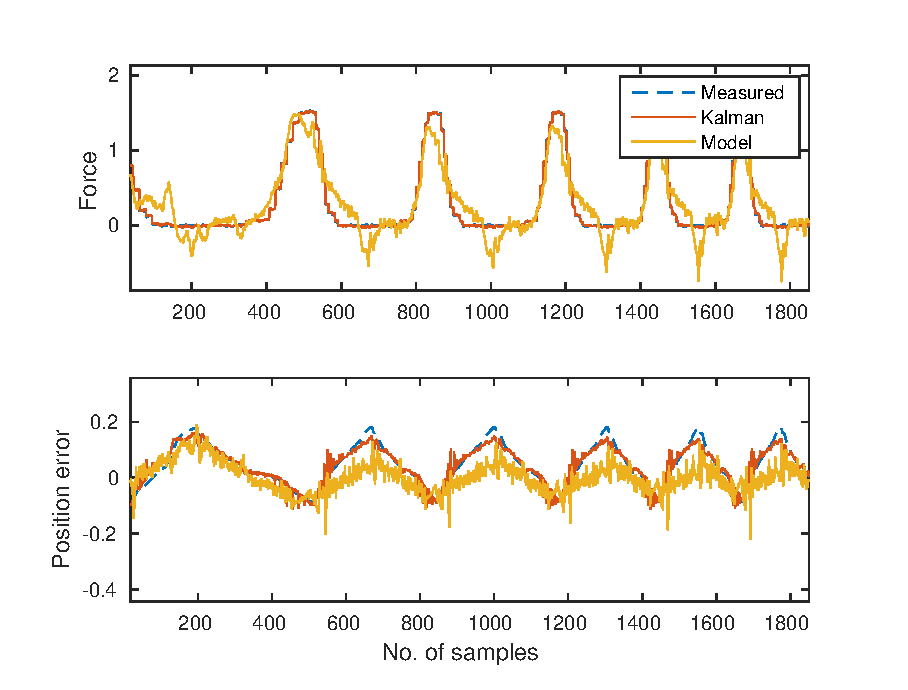
\includegraphics[width=0.49\linewidth]{kl1}
\hspace{-2.5em}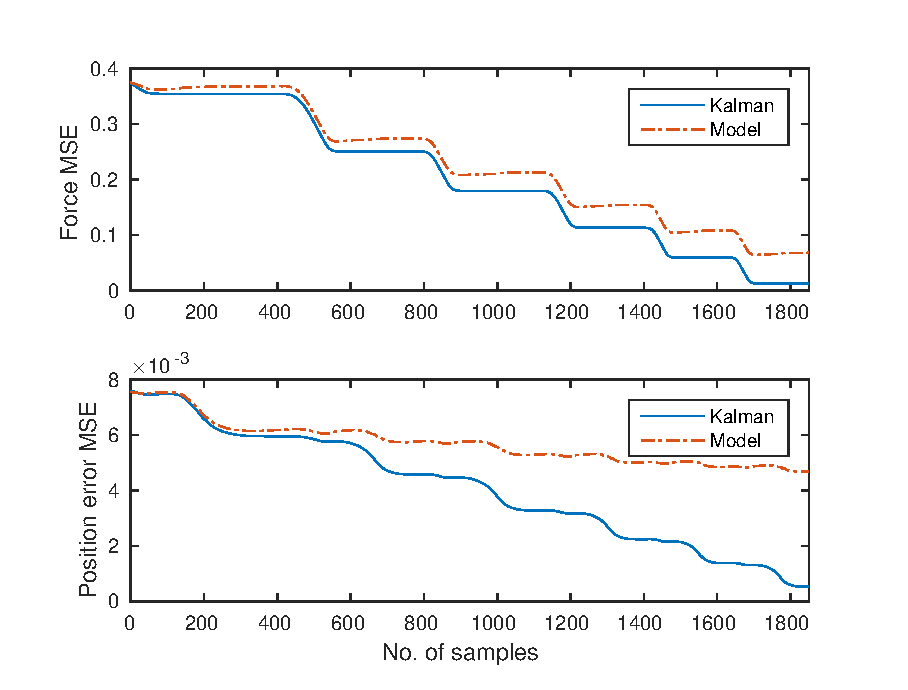
\includegraphics[width=0.49\linewidth]{kl1mse}
\caption{Left: Response of the model and the filter estimate compared to measurments. Right: Comparison of mean-square errors.}
\label{fig:kl1}
\end{figure}

As seen on (\figref{kl1}), the Kalman filter surpasses the open-loop model when all the measurements are available.
Both the force and position error estimates havea really low error which can be reduced further by recalculating the gain for higher values in the $\mathbf{Q}$ matrix.
With this proof of concept, the same simulation is attempted for only the position error measurement.

\begin{figure}[H]
\centering
\hspace{-2.5em}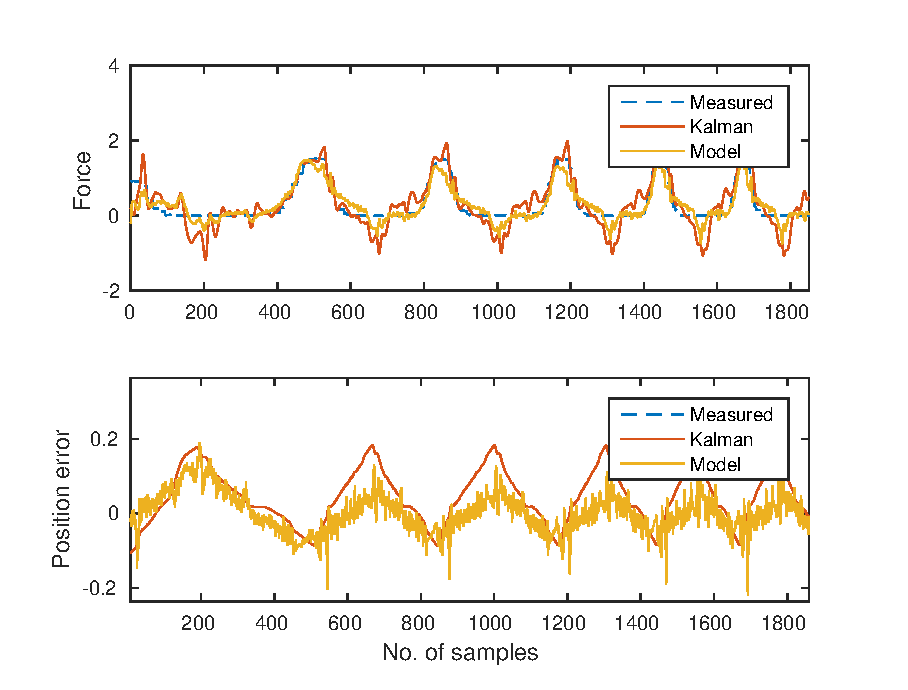
\includegraphics[width=0.49\linewidth]{kl2}
\hspace{-2.5em}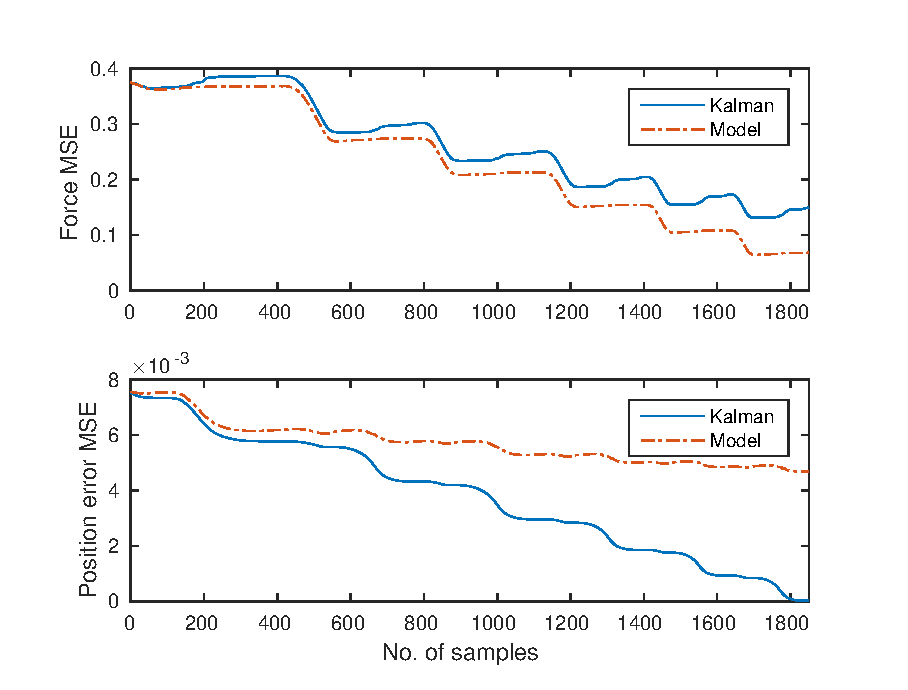
\includegraphics[width=0.49\linewidth]{kl2mse}
\caption{Left: Response of the model and the filter estimate compared to measurments. Right: Comparison of mean-square errors.}
\label{fig:kl2}
\end{figure}

As seen on \figref{kl2}, when the only measurement is the position error, system state estimation isn't nearly as accurate.
The states are estimated in a way that makes the position error output converge twoards the measurments, but it doesn't reduce (or significantly increase) the force estimate error.
It is concluded that this is mostly to the lack of accuracy in the model itself, and as such a Kalman filter wouldn't bring any advantages to the system.
Nontheless, the Kalman filter is included in the software implementation, so that higher accuracy models can be tested.

%\begin{figure} 
%	\resizebox{\textwidth}{!}{
%		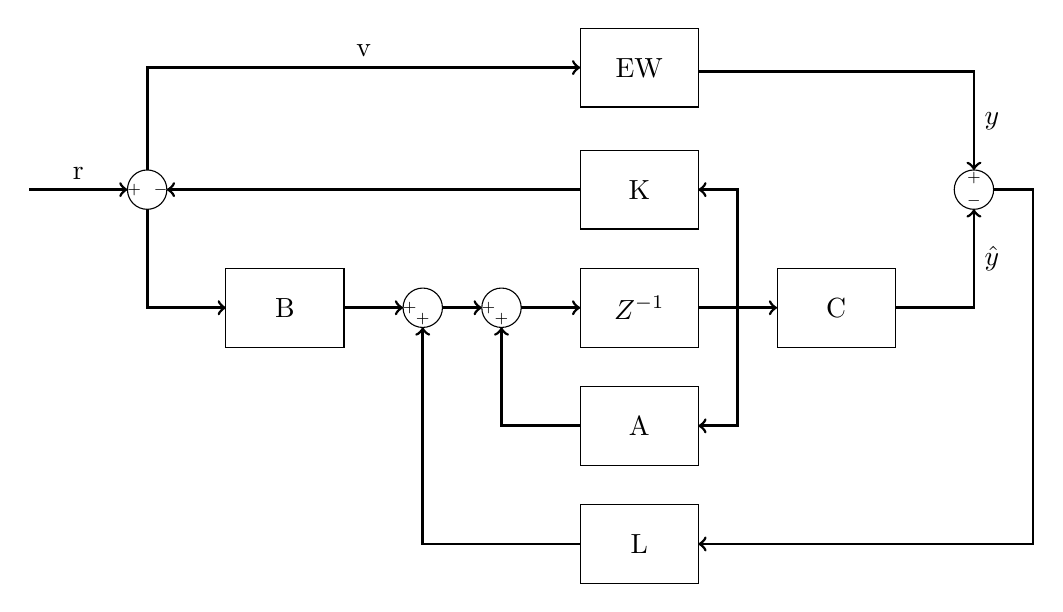
\begin{tikzpicture}
\draw  (0,0) rectangle (1.5,1)node[pos=0.5]{L};
\draw  (0,1.5) rectangle (1.5,2.5)node[pos=0.5]{A};
\draw  (0,3) rectangle (1.5,4)node[pos=0.5]{$Z^{-1}$};
\draw  (0,4.5) rectangle (1.5,5.5)node[pos=0.5]{K};
\draw  (0,6.05) rectangle (1.5,7.05)node[pos=0.5]{EW};
\draw  (2.5,3) rectangle (4,4)node[pos=0.5]{C};
\draw  (-4.5,3) rectangle (-3,4)node[pos=0.5]{B};
\draw  (-1,3.5) ellipse (0.25 and 0.25) node  [ left=-0.5mm]{\tiny$+$} node  [below =-0.5mm]{\tiny$+$};
\draw  (-2,3.5) ellipse (0.25 and 0.25) node  [ left=-0.5mm]{\tiny$+$} node  [below =-0.5mm]{\tiny$+$};
\draw  (5,5) ellipse (0.25 and 0.25) node  [ above=-0.5mm]{\tiny$+$} node  [below =-0.5mm]{\tiny$-$};
\draw  (-5.5,5) ellipse (0.25 and 0.25) node  [ left=-0.5mm]{\tiny$+$} node  [right =-0.5mm]{\tiny$-$};

\draw [->,line width=1] (0,2) -- (-1,2) -- (-1,3.25);
\draw  [->,line width=1](0,0.5) -- (-2,0.5) -- (-2,3.25);
\draw   [->,line width=1](-3,3.5) -- (-2.25,3.5);
\draw   [->,line width=1](-1.75,3.5) -- (-1.25,3.5);
\draw   [->,line width=1](-0.75,3.5) -- (0,3.5);
\draw [->,line width=1](1.5,3.5) -- (2.5,3.5);
\draw [->,line width=1](2,3.5) node (v1) {} -- (2,2) -- (1.5,2);
\draw [->,line width=1](4,3.5) -- (5,3.5) --  node[right, pos=0.5]{$\hat y$}(5,4.75);
\draw [->,line width=1](2,3.5) -- (2,5) -- (1.5,5);
\draw [->,line width=1](5.25,5) -- (5.75,5) -- (5.75,0.5) -- (1.5,0.5);
\draw [->,line width=1](1.5,6.5) -- (5,6.5) -- node[right, pos=0.5]{$y$}(5,5.25);
\draw [->,line width=1](0,5) -- (-0.95,5) -- (-5.25,5);
\draw [->,line width=1](-5.5,5.25)--(-5.5,6.55) --  node[above, pos=0.5]{v}(0,6.55);
\draw  [->,line width=1](-7,5) -- (-5.75,5)node[above, pos=0.5]{r};
\draw [->,line width=1](-5.5,4.75) -- (-5.5,3.5) -- (-4.5,3.5);
\end{tikzpicture}
%	}
%	\caption{Block diagram of a Hammerstein-Wiener model.}
%	\label{weiner}
%\end{figure}
%\todo{nice figure, what is it for?}